% ==============================================================================
% FICHIER : chapitre2.tex
% Description : Chapitre 2 : Planification & architecture
% Auteurs : Dhia Fersi & Mohamed Iyed Amiri (ISET Bizerte)
% Organisme d'accueil : HRMAPS
% ==============================================================================

\chapter{Planification \& architecture}

\section*{Introduction}
\addcontentsline{toc}{section}{Introduction}
La réussite d'un projet informatique complexe repose sur une planification rigoureuse et une architecture logicielle bien pensée. Pour développer \textit{SafeCity-Connect}, nous avons adopté la méthodologie agile \textbf{SCRUM}, réputée pour sa flexibilité et son efficacité de développement. Ce chapitre détaille la spécification des besoins de notre système, présente notre équipe SCRUM, définit le découpage des sprints, expose le Backlog de produit global, et introduit la modélisation fonctionnelle et structurelle à travers les diagrammes UML globaux.

% ------------------------------------------------------------------------------
% 1. SPÉCIFICATION DES BESOINS
% ------------------------------------------------------------------------------
\section{Spécification des besoins}

\subsection{Identification des acteurs du système}
Nous avons identifié quatre acteurs principaux qui interagissent avec la plateforme :
\begin{itemize}
    \item \textbf{Le Citoyen} : Utilise l'application mobile Flutter pour signaler des incidents géolocalisés avec photo, suivre le statut de résolution (fixé ou non) directement sur la carte, laisser des commentaires, et donner son avis sur la réparation finale (\textit{review fixes}).
    \item \textbf{L'Administrateur municipal} : Utilise l'application web Angular pour gérer Keycloak (créer/gérer les comptes des Départements), affecter les interventions, valider/rejeter les preuves de fixation (avec motif obligatoire), analyser la Heatmap, suivre la timeline d'évolution détaillée, recevoir des e-mails d'alertes lors de nouveaux signalements, et exporter les rapports hebdomadaires et fiches d'incidents sous format PDF.
    \item \textbf{Le Département municipal (Agent d'intervention)} : Utilise l'application mobile Flutter pour se connecter via un compte créé par l'admin, consulter ses missions de voirie affectées, effectuer les travaux et soumettre la photo preuve de résolution sur site.
    \item \textbf{Le Système d'IA (YOLO)} : Traite l'image soumise pour classifier automatiquement l'incident.
\end{itemize}

\subsection{Les besoins fonctionnels}
Les besoins fonctionnels décrivent les capacités opérationnelles que doit fournir le système :
\begin{itemize}
    \item \textbf{Gestion d'Identité et Rôles} : Inscription/connexion SSO (Keycloak) pour les citoyens et agents techniques (les comptes Département étant créés manuellement par l'Administrateur).
    \item \textbf{Signalement \& IA (Citoyen)} : Envoi de signalement (photo, localisation Leaflet, classement automatique par YOLO).
    \item \textbf{Commentaires et Revue (Citoyen)} : Ajout de commentaires sur les incidents et validation ou avis après résolution (\textit{review fixes}).
    \item \textbf{Timeline d'Évolution (Admin)} : Fil de vie historique complet (soumission, affectation, réparation, validation/rejet) pour chaque incident, accessible uniquement par l'Administrateur.
    \item \textbf{Affectation \& Modération (Admin)} : Transmission du problème au département idoine ; vérification de la preuve de fixation avec droit d'acceptation ou de rejet motivé (raison obligatoire).
    \item \textbf{Reporting \& Export (Admin)} : Tableau de bord analytique, export hebdomadaire (Excel) et génération de rapports de synthèse au format PDF.
    \item \textbf{Alertes Système} : Envoi instantané d'une notification e-mail à l'Admin lors d'un nouveau signalement citoyen.
    \item \textbf{Opérations terrain (Département)} : Consultation des tâches affectées et transmission de la photo preuve de résolution.
\end{itemize}

\subsection{Les besoins non fonctionnels}
Les besoins non fonctionnels décrivent les caractéristiques de qualité de notre plateforme :
\begin{itemize}
    \item \textbf{Sécurité} : Authentification OAuth2/OIDC gérée centralement par Keycloak pour sécuriser les flux de données.
    \item \textbf{Performance} : Rendu fluide et rapide de la carte thermique et des points, même avec un grand nombre d'incidents (grâce aux index GIST spatiaux sous PostGIS).
    \item \textbf{Ergonomie} : Interface adaptative (\textit{responsive}) respectant les standards du mobile-first pour faciliter l'utilisation sur le terrain.
\end{itemize}

% ------------------------------------------------------------------------------
% 2. STRUCTURE ET DÉCOUPAGE DU PROJET
% ------------------------------------------------------------------------------
\section{Structure et découpage du projet}

\subsection{Identification de l'équipe SCRUM}
L'organisation de notre projet s'articule autour des rôles SCRUM suivants :
\begin{itemize}
    \item \textbf{Product Owners} : Dhia Fersi \& Mohamed Iyed Amiri (en collaboration avec l'encadrant professionnel Rami Bouafif de HRMAPS qui a spécifié les priorités).
    \item \textbf{Scrum Masters} : Dhia Fersi \& Mohamed Iyed Amiri (partage du rôle pour orchestrer le projet).
    \item \textbf{Équipe de Développement} : Dhia Fersi (spécialisé Backend \& PostGIS / IA) \& Mohamed Iyed Amiri (spécialisé Frontend Angular \& Leaflet / Keycloak).
\end{itemize}

\subsection{Découpage des sprints}
Afin de livrer régulièrement des incréments logiciels fonctionnels, nous avons découpé le projet en 5 sprints majeurs (chacun d'une durée de 2 semaines) :
\begin{itemize}
    \item \textbf{Sprint 0} : Mise en place de l'architecture logicielle, infrastructure Docker et technologies de développement.
    \item \textbf{Sprint 1} : Inscription, Authentification unifiée, Gestion de profil et Sécurité via Keycloak.
    \item \textbf{Sprint 2} : Espace Citoyen -- Gestion des Signalements, intégration cartographique Leaflet et analyse photo IA (YOLO).
    \item \textbf{Sprint 3} : Espace Administration -- Tableau de bord, Carte de chaleur spatiale (\textit{Heatmap}) PostGIS et outils de statistiques.
    \item \textbf{Sprint 4} : Espace Gamification -- Historique citoyen, gestion des points d'impact et validation globale.
\end{itemize}

\subsection{Le Backlog du produit}
Le tableau \ref{tab:backlog_produit} résume les récits utilisateurs (\textit{User Stories}) du Backlog Produit :

\begin{table}[H]
    \centering
    \caption{Backlog de Produit SafeCity-Connect}
    \label{tab:backlog_produit}
    \vspace{0.2cm}
    \small
    \begin{tabularx}{\textwidth}{l p{7.5cm} c c c}
        \toprule
        \textbf{ID} & \textbf{User Story (En tant que... Je veux... Afin de...)} & \textbf{Priorité} & \textbf{Complexité} & \textbf{Sprint} \\
        \midrule
        \textbf{US01} & Déployer l'architecture globale conteneurisée. & Haute & 5 & Sprint 0 \\
        \textbf{US02} & M'inscrire, me connecter et gérer mon profil (Citoyen/Dept). & Haute & 8 & Sprint 1 \\
        \textbf{US03} & Créer et gérer les comptes des agents techniques (Admin). & Moyenne & 3 & Sprint 1 \\
        \textbf{US04} & Signaler un incident avec géo-localisation et photo IA. & Haute & 13 & Sprint 2 \\
        \textbf{US05} & Consulter le statut de résolution (fixé/non fixé) sur la carte. & Haute & 3 & Sprint 2 \\
        \textbf{US06} & Affecter des incidents aux départements techniques (Admin). & Haute & 5 & Sprint 3 \\
        \textbf{US07} & Exporter les incidents hebdomadaires et fiches PDF (Admin). & Moyenne & 8 & Sprint 3 \\
        \textbf{US08} & Recevoir des alertes par e-mail lors de signalements. & Moyenne & 5 & Sprint 3 \\
        \textbf{US09} & Uploader une photo preuve de résolution (Département). & Haute & 8 & Sprint 4 \\
        \textbf{US10} & Accepter ou rejeter la fixation avec motif (Admin). & Haute & 8 & Sprint 4 \\
        \textbf{US11} & Échanger des commentaires et évaluer les réparations (Citoyen). & Moyenne & 8 & Sprint 4 \\
        \bottomrule
    \end{tabularx}
\end{table}

\subsection{Planification des releases}
Notre projet prévoit une release intermédiaire après le Sprint 2 (version citoyenne fonctionnelle avec signalement IA) et une release finale de production à la fin du Sprint 4 (version complète avec dashboard d'administration et de gamification).

\subsection{Diagramme de cas d'utilisation global}
Le diagramme de cas d'utilisation global modélise l'ensemble des interactions fonctionnelles autorisées pour chaque acteur (voir Figure \ref{fig:uc_global}).

\begin{figure}[H]
    \centering
    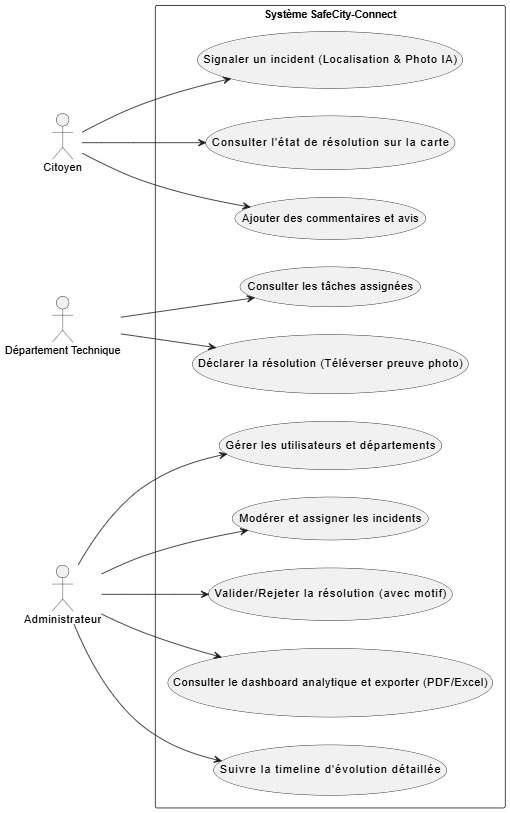
\includegraphics[width=0.9\textwidth]{use_case_global.jpg}
    \caption{Diagramme de cas d'utilisation global de la plateforme}
    \label{fig:uc_global}
\end{figure}

\subsection{Diagramme de classe global (initial)}
Le diagramme de classe global initial présente la structure conceptuelle des données et les relations métiers qui seront stockées en base de données (voir Figure \ref{fig:classes_global}).

\begin{figure}[H]
    \centering
    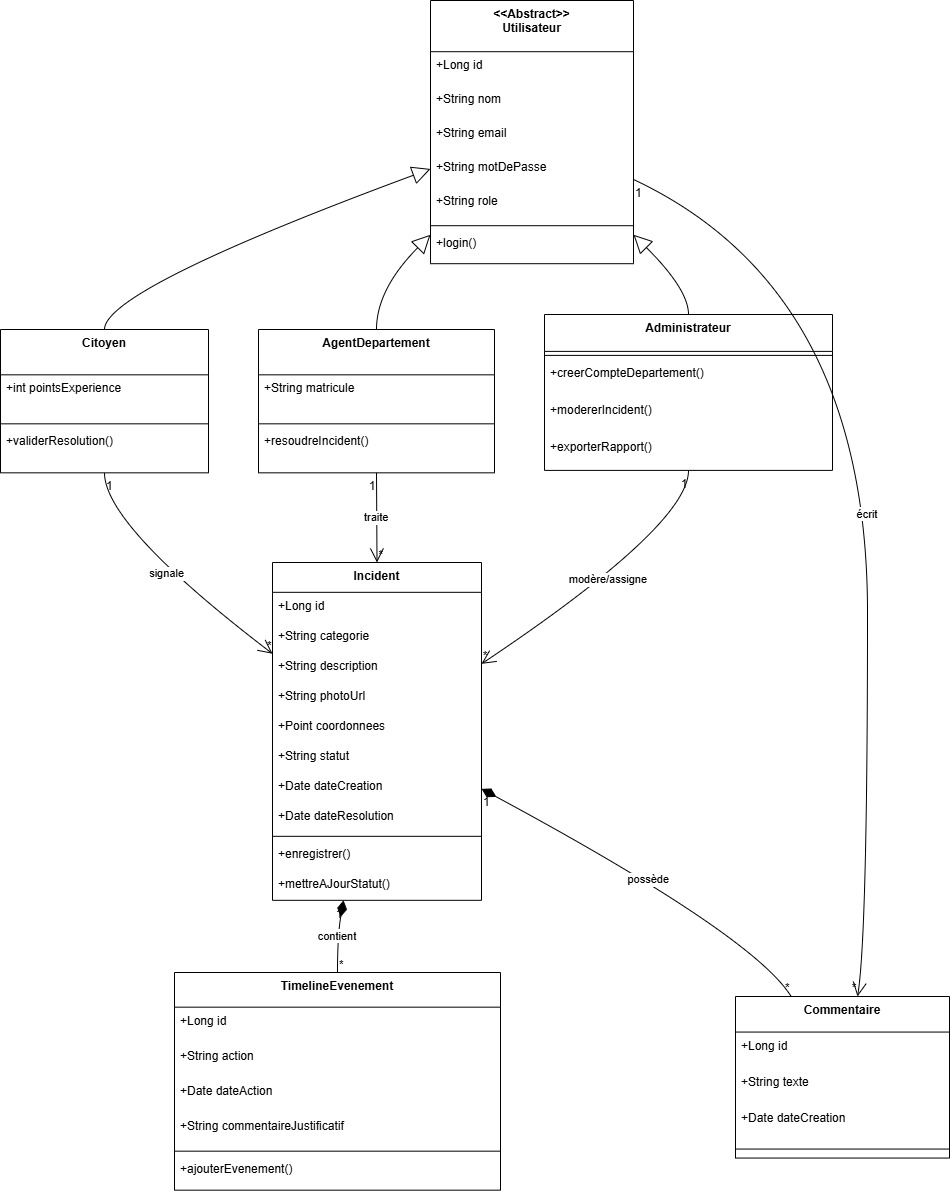
\includegraphics[width=0.9\textwidth]{classes_global.jpg}
    \caption{Diagramme de classes global initial}
    \label{fig:classes_global}
\end{figure}

\section*{Conclusion}
\addcontentsline{toc}{section}{Conclusion}
Ce deuxième chapitre nous a permis de structurer la planification agile du projet en identifiant l'équipe SCRUM, en découpant le projet en Sprints opérationnels, et en formalisant le Backlog de produit. Nous avons également établi la modélisation fonctionnelle et conceptuelle globale de \textit{SafeCity-Connect}. Le chapitre suivant détaillera le Sprint 0, consacré à la mise en place de notre architecture logicielle et de nos outils de développement.
